%
% thesis
% @author Tobias Weber <tweber@ill.fr>
% @date jan-2021
% @license see 'LICENSE' file
%

\documentclass[english, 11pt]{book}

\RequirePackage{fixltx2e}
\RequirePackage{fix-cm}

\usepackage{amsmath}
\usepackage{tensor}
\usepackage{bm}
\usepackage{graphicx}
\usepackage{siunitx}
\usepackage{babel}
\usepackage[hyphens]{url}
\usepackage[numbib, chapter]{tocbibind}
\usepackage[colorlinks=true, linkcolor=black, citecolor=blue, urlcolor=blue, unicode=true]{hyperref}
\usepackage[a4paper]{geometry}
\geometry{tmargin=2.5cm, bmargin=2.5cm, lmargin=2cm, rmargin=2cm}

\renewcommand{\arraystretch}{1.25}

\makeatletter
% Bold math tip from Prof. Icking and https://tex.stackexchange.com/questions/209466/problem-with-tocloft-minitoc-and-bold-math-mode
\g@addto@macro\bfseries{\mathversion{bold}}
\makeatother


\begin{document}

\newcommand{\ill}{Institut Laue-Langevin (ILL), 71 avenue des Martyrs, CS 20156, 38042 Grenoble cedex 9, France}
\newcommand{\fuh}{Fernuniversit\"at in Hagen (FUH), Universit\"atsstraße 47, 58097 Hagen, Germany}


\title{Path-finding for triple-axis spectrometers}
\author{Tobias Weber, tweber@ill.fr}

\maketitle
\tableofcontents




% ====================================================================================================================================
%\part{Front matter}
%\addcontentsline{toc}{part}{Front matter} 
%
% project plan / abstract
% @author Tobias Weber <tweber@ill.fr>
% @date jan-2021
% @license see 'LICENSE' file
%

\chapter*{Abstract}
\addcontentsline{toc}{chapter}{Abstract}

The triple-axis spectrometer (TAS) \cite{Shirane2002} was invented by B. Brockhouse in the 1950s and 
is among the foremost measurement methods in the field of inelastic neutron scattering. 
It enables the probing of vibrational (phonon) or magnetic (magnon) excitations in single crystals and allows 
mappings of their dispersion relations, i.e. their energy-momentum relation, $E\left( \bm{Q} \right)$.

The three axes of a TAS are offset by relative angles to one another, and comprise 
(i) the reactor-monochromator-sample axis, where a specific neutron energy is picked out of the polychromatic 
beam coming from the reactor's moderator; 
(ii) the monochromator-sample-analyser axis, whose angle selects a specific momentum transfer, $\bm{Q}$, 
from the neutron to the sample; and 
(iii) the sample-analyser-detector axis, which selects the energy transfer, $E$.

During the usual operation of a TAS, the user selects $\left( \bm{Q}, E \right)$ coordinates in the reciprocal (dual)
crystal space of the sample to be measured. While the vector space of crystal coordinates 
is in general non-Euclidean, crystal coordinates have a one-to-one correspondence with the axis angles 
of the TAS. The correspondence can be calculated by the so-called ``$UB$ matrix formalism'' \cite{Lumsden2005}. 
Here, $B$ is the transformation matrix from crystal to lab coordinates and $U$ is a rotation to a specific 
crystal plane. From that, the TAS angles can be derived using Bragg's law.

Due to angular constraints by cables and tubes, as well as spatial constraints from the crammed instrument space, 
not every $\left( \bm{Q}, E \right)$ coordinate point is accessible, and a careful mapping of each point is
usually required beforehand to avoid collisions of the instrument with walls, collisions with itself or movements
which could pull out fragile cables.

The goal of the proposed project is the development and implementation of a path-finding algorithm for 
neutron triple-axis spectrometers. Given a user-selected target coordinate in reciprocal crystal space, 
the algorithm will be able to navigate the instrument in its constrained angular space. The problem is similar to 
moving a robot arm around obstacles, with the addition of having the start and target coordinates in a 
coordinate system with a different metric.

%\begin{figure}[ht]
%	\begin{centering}
%	\includegraphics[width=0.66\textwidth]{figures/thales.jpg}
%	\end{centering}
%	\caption{The picture shows the triple-axis spectrometer \textit{ThALES} \cite{thales} at the ILL.}
%	\label{fig:tas}
%\end{figure}

%
% acknowledgements and thanks
% @author Tobias Weber <tweber@ill.fr>
% @date july-2021
% @license see 'LICENSE' file
%

\chapter*{Acknowledgements}
\addcontentsline{toc}{chapter}{Acknowledgements and Thanks}

I wish to thank my thesis advisors, Prof. Dr. Christian Icking and Dr. Lihong Ma, for accepting 
and supporting this project, for their advice and our regular discussions, the friendly atmosphere, 
as well as for always being available for questions.

Equal thanks to Dr. Martin B\"ohm, leader of the spectroscopy group at the ILL and instrument 
scientist at the \textit{Thales} spectrometer, to Yannick Le Goc (computer scientist at the instrument 
control and electronics group), as well as Dr. Paul Steffens (\textit{Thales} instrument scientist) for our 
regular discussions about various triple-axis automatisation projects, our experiments and the
instrumental aspects. I furthermore wish to thank Jérôme Locatelli (instrument control group) for
all the help with \textit{NOMAD}, the instrument control system at the ILL, and the technical discussions
about its internal details. 
Thanks to Dr. Paolo Mutti, the head of both the scientific computing and the instrument control group 
at the ILL, for supporting this project and for the great atmosphere and working environment there.

Also not to forget the continuing support from my former advisor for past theses, Prof. Dr. Peter B\"oni,
as well as from Prof. Dr. Christian Pfleiderer, Prof. Dr. Markus Garst, and Dr. Marc Janoschek in all our ongoing projects.

Financial support by the Institut Laue-Langevin via its \textit{P\^ole Formation} is gratefully acknowledged,
an I wish to thank Carole Fauchier for the administrative help.

Last but not least also many thanks to my family and to Soilhat for always being there for me!



%\part{Main part}

\chapter{Introduction}
In this chapter we introduce the concepts of neutron scattering and shortly present the different types of instruments typically found at a research reactor (Sec. \ref{sec:scattering}). A special emphasis is put on triple-axis spectrometers (TAS) as the work-horse of inelastic scattering (Sec. \ref{sec:scattering}). Finally, we summarise the current state of autonomous experimentation (Sec. \ref{sec:autonomous}).



\section{Neutron scattering \label{sec:scattering}}

The history of neutron physics begins in 1932 with the discovery of the neutron by James Chadwick, who used alpha particles (helium nuclei) to bombard a beryllium-9 sample, thereby producing carbon-12 and one neutron per reaction \cite[p.1]{Jacrot2021}. The neutron was found to have a similar mass as the proton ($m_n = 1.675\cdot10^{-27}\,\mathrm{kg}$, $m_p = 1.673\cdot10^{-27}\,\mathrm{kg}$), but, as the name implies, does not possess a charge \cite[p. 2]{Squires2012}. The absence of a charge makes the neutron very useful for science, as it is subject to purely nuclear interactions with other nuclei, without any electrostatic repulsion \cite[p. 1]{Squires2012}.

In 1939, Otto Hahn used a Chadwick-type neutron source to irradiate uranium isotopes in an attempt to produce heavy trans-uranium elements \cite{wiki_fission}. But instead of heavier elements, the experiment yielded lighter elements, which was interpreted by Lise Meitner as a splitting of the uranium nucleus, the discovery of nuclear fission \cite{wiki_fission}. A typical possible channel of a fission reaction is the decay of uranium-235 into baryum-144 and krypton-89, where two to three neutrons are produced by each reaction in addition to the daughter nuclei and energy \cite{wiki_fission}.

In 1942, Enrico Fermi made use of the excess neutrons that are obtained by each fission reaction to produce a continuous, self-sustaining chain reaction in the first artificial nuclear reactor, the \textit{Chicago Pile-1}~\cite[p.1]{Jacrot2021}~\footnote{Note that \textit{Chicago Pile-1} was the first \textit{artificial} nuclear reactor. The first \textit{natural} reactor was discovered to have run more that 1.5 billion years ago in Oklo, Gabun, at an average power of about 100 kW for a period of half a million years \cite{wiki_oklo}.}.

The first research reactor, having a power of 3.5 MW~\footnote{As research reactors do not produce electricity, the given numbers refer to thermal powers.} and being used for studies in solid-state physics, was built in Oak Ridge, USA in 1943, shortly after Fermi's pile \cite[p.3]{Jacrot2021}. 
Here, first neutron scattering experiments were performed by Clifford Shull using a two-axis diffractometer \cite[p.3]{Jacrot2021}.

A two-axis diffractometer is used for studying the structure of crystals. This is possible, because neutrons coming from the reactor can be slowed down (moderated) into energy regions where their de Broglie wavelength $\lambda = h/p$ corresponds to typical inter-atomic distances in crystal unit cells, which is of the order of 1 \AA{}ngstr\"om, i.e. $10^{-10}$ m \cite[pp.1,3]{Squires2012}.



\section{Triple-axis spectrometers \label{sec:tas}}

The triple-axis spectrometer (TAS) is one of the fundamental types of instruments in the field of neutron scattering at research reactors.

\clearpage
\begin{figure*}[htb]
	\centering
	\includegraphics[width=0.75\textwidth]{figures/thales.jpg}
	\caption{The triple-axis spectrometer ThALES \cite{thales} at the Institut Laue-Langevin in Grenoble, France. This picture is reproduced from \cite{TODO}.}
	\label{fig:thales}
\end{figure*}



\section{Autonomous experiments \label{sec:autonomous}}

The goal of this work is the design and implementation of software tools which enable an automatic path finding for TAS instruments.
Automatic path finding is necessary for the instrument to circumvent obstacles in its path. The methods in this work are part of the current drive towards autonomous experimentation.


\chapter{Crystal and Instrument Coordinate Systems}
\label{ch:xtal}
%
% xtal formulas
% @author Tobias Weber <tweber@ill.fr>
% @date 13-jul-2018
% @license see 'LICENSE' file
%

\chapter{Crystal and Instrument Coordinate Systems}
\label{ch:xtal}

In this chapter we review the theory for conversion between crystal coordinates and scattering angles at the triple-axis instrument. Section \ref{sec:xtalcoords} introduces crystal coordinates and the so-called UB matrix formalism, section \ref{sec:tasangles} calculates the corresponding TAS angles. Note this chapter has been published in the manual of the software from Ref. \cite{Takin2021} and is based on an earlier version of these derivations from my (physics) PhD thesis \cite[pp. 139-143]{PhDWeber}.


% ------------------------------------------------------------------------------------------------------------------------------------
\section{Fractional crystal coordinates \label{sec:xtalcoords}}

We begin by presenting the so-called $UB$ matrix formalism to convert between relative lattice units of a crystal and laboratory coordinates used in instrument space. This method has been described in \cite{Lumsden2005}. The derivation of the transformation matrices, $A$ and $B$, describing fractional crystal coordinates, can be found in \cite{wiki_fractional}, which we follow here.

\subsection{$A$ and $B$ matrices}
The unit cell of the crystal is spanned by its three basis vectors $\left| a \right>$, $\left| b \right>$, and $\left| c \right>$, which -- in general -- are not perpendicular to one another, but instead enclose angles of $\alpha$, $\beta$, and $\gamma$, respectively, as shown in Fig. \ref{fig:cell}. 
To calculate the crystallographic $A$ matrix which transforms non-orthogonal crystal to orthogonal lab units, we first need to reduce the number of parameters.
The respective relations between the basis vectors and their angles can be directly obtained via the cosine theorem:
\begin{equation} \left< a | b \right > \ =\  ab \cos \gamma, \label{ab} \end{equation}
\begin{equation} \left< a | c \right > \ =\  ac \cos \beta, \label{ac} \end{equation}
\begin{equation} \left< b | c \right > \ =\  bc \cos \alpha. \label{bc} \end{equation}

\begin{figure}
	\centering
	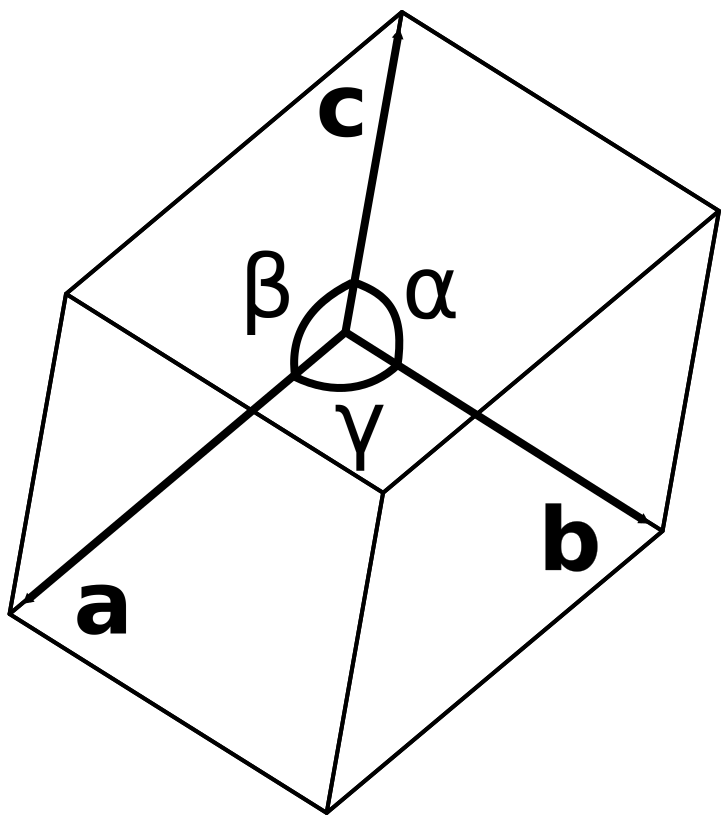
\includegraphics[width = 0.2 \textwidth]{figures/cell}
	\caption[Crystal unit cell.]{
		The unit cell of a crystal is given by its coordinate vectors $a$, $b$, and $c$ 
		as well as their angles $\alpha$, $\beta$, and $\gamma$.}
	\label{fig:cell}
\end{figure}


%\subsection*{Basis vectors}

The next goal is to explicitly write the components of the vectors $\left| a \right>$, $\left| b \right>$, and $\left| c \right>$ in terms of their (scalar) lengths $a = \sqrt{\left< a | a \right>}$, $b = \sqrt{\left< b | b \right>}$, $c = \sqrt{\left< c | c \right>}$, and the three angles.
To that end, we first choose -- without loss of generality -- $\left| a \right>$ along the $x$ axis, $\left| b \right>$ in the $xy$ plane, and $\left| c \right>$ in general:
\begin{equation} 
	\boxed{ \left| a \right> \ =\  \left( \begin{array}{c} a_1 = a \\ 0 \\ 0 \end{array} \right), }
	\hspace{0.5cm} \left| b \right> \ =\  \left( \begin{array}{c} b_1 \\ b_2 \\ 0 \end{array} \right),
	\hspace{0.5cm} \left| c \right> \ =\  \left( \begin{array}{c} c_1 \\ c_2 \\ c_3 \end{array} \right).
\end{equation}


Inserting $\left| a \right>$ and $\left| b \right>$ into Eq. \ref{ab} gives:

\begin{equation} \left< a | b \right > \ =\  a_1 b_1 \ =\  ab \cos \gamma, \end{equation}
\begin{equation} b_1 \ =\  b \cos \gamma. \end{equation}


Using the cross product between $\left| a \right>$ and $\left| b \right>$, we get:
\begin{equation} 
	\left\Vert \left| a \right> \times \left| b \right> \right\Vert \ =\ 
	\left\Vert \left( \begin{array}{c} 0 \\ 0 \\ a_1 b_2 \end{array} \right) \right\Vert \ =\ 
	ab \sin \gamma, \label{crossab}
\end{equation}
\begin{equation} b_2 \ =\  b \sin \gamma, \end{equation}
\begin{equation} 
\boxed{ \left| b \right> \ =\  \left( \begin{array}{c} b \cos \gamma \\ b \sin \gamma \\ 0 \end{array} \right). } 
\label{bvec} 
\end{equation}


Inserting $\left| a \right>$ and $\left| c \right>$ into Eq. \ref{ac} gives:

\begin{equation} \left< a | c \right > \ =\  a_1 c_1 \ =\  ac \cos \beta, \end{equation}
\begin{equation} c_1 \ =\  c \cos \beta. \end{equation}



Inserting $\left| b \right>$ and $\left| c \right>$ into Eq. \ref{bc} gives:

\begin{equation} \left< b | c \right > \ =\  b_1 c_1 + b_2 c_2 \ =\  bc \cos \alpha, \end{equation}
\begin{equation} b \cos \gamma \cdot c \cos \beta + b \sin \gamma \cdot c_2 \ =\  bc \cos \alpha, \end{equation}
\begin{equation} c_2 \ =\  \frac{c \cos \alpha - c \cos \gamma \cos \beta}{\sin \gamma}. \end{equation}



The last component, $c_3$, can be obtained from the vector length normalisation, $ \left< c | c \right> = c^2 $:
\begin{equation} \left< c | c \right > \ =\  c_1^2 + c_2^2 + c_3^2 \ =\  c^2, \end{equation}
\begin{equation} c_3^2 \ =\  c^2 - c_1^2 - c_2^2, \end{equation}
\begin{equation} 
	c_3^2 \ =\  c^2 \left[1 - \cos^2 \beta - \left(\frac{\cos \alpha - \cos \gamma \cos \beta}{\sin \gamma} \right)^2 \right], 
\end{equation}
\begin{equation} \boxed{ \left| c \right> \ =\  \left( \begin{array}{c}
	c \cdot \cos \beta \\
	c \cdot \frac{\cos \alpha - \cos \gamma \cos \beta}{\sin \gamma} \\
	c \cdot \sqrt{ \sin^2 \beta - \left(\frac{\cos \alpha - \cos \gamma \cos \beta}{\sin \gamma} \right)^2 }
\end{array} \right). } \end{equation}



The crystallographic $A$ matrix, which transforms real-space fractional to lab coordinates (\AA), is formed with the basis vectors in its columns:
\begin{equation}
	A \ =\  \left(
		\begin{array}{ccc}
			\left| a \right> & \left| b \right> & \left| c \right>
		\end{array}
	\right).
\end{equation}
Explicitly written out using the basis vectors, the matrix reads \cite{wiki_fractional}:
\begin{equation}
	A \ =\  \left(
		\begin{array}{ccc}
			\begin{array}{c} a \\ 0 \\ 0 \end{array}
			& 
			\begin{array}{c} b \cos \gamma \\ b \sin \gamma \\ 0 \end{array} 
			& 
			\begin{array}{c}
				c \cdot \cos \beta \\
				c \cdot \frac{\cos \alpha - \cos \gamma \cos \beta}{\sin \gamma} \\
				c \cdot \sqrt{ \sin^2 \beta - \left(\frac{\cos \alpha - \cos \gamma \cos \beta}{\sin \gamma} \right)^2 }
			\end{array}
		\end{array}
	\right).
\end{equation}


The $B$ matrix, which transforms reciprocal-space relative lattice units (rlu) to lab coordinates (1/\AA), is:
\begin{equation} B \ =\  2 \pi A^{-t}, \end{equation}
where $-t$ denotes the transposed inverse.
We can now also determine the metric tensor corresponding to the coordinate system defined by the $B$ transformation matrix, it reads \cite[p. 808]{Arens2015}:
\begin{equation}
	\left(g_{ij}\right) \ =\  \left<\underline{b}_i | \underline{b}_j \right> \ =\  B^T B,
\end{equation}
where the reciprocal basis vectors $\left| \underline{b}_i \right>$ form the columns of $B$.


\subsection{Example: lengths and angles in the reciprocal lattice}
Having a metric makes it straightforward to calculate lengths and angles.
The length of a reciprocal lattice vector $\left| G \right>$ seen from the lab system is (in 1/\AA{} units) \cite[p. 808]{Arens2015}:
\begin{equation}
	\left\Vert \left< G | G \right> \right\Vert \ =\  \sqrt{\left< G | G \right>} \ =\  \sqrt{G_i G^i} \ =\  \sqrt{g_{ij} G^i G^j}.
\end{equation}
The angle $\theta$ between two Bragg peaks $\left| G \right>$ and $\left| H \right>$ is given by their dot product \cite[p. 808]{Arens2015}:
\begin{equation}
	\frac{\left< G | H \right>}{\left\Vert \left< G | G \right> \right\Vert \cdot \left\Vert \left< H | H \right> \right\Vert} \ =\  
	\frac{g_{ij} G^i H^j }{\sqrt{g_{ij} G^i G^j} \sqrt{g_{ij} H^i H^j}} \ =\  \cos \theta.
\end{equation}

Please note that if an index appears twice, both as subscript as well as a superscript, a summation over it is implied, see Ref. \cite{wiki_summation}.


\subsection{$U$ matrix}
The $B$ matrix alone yields the transformation from the non-orthogonal and reciprocal crystal coordinate system into the orthogonal lab units.
However, it does not yet take into account the actual rotation of the crystal so that a specific plane, the so-called scattering plane, 
can be accessed by the two-dimensional movements of the instrument. 
Such a rotation is performed by the $U$ matrix, whose rows contain two vectors inside the desired scattering plane and the plane normal. 
These basis vectors are usually chosen along two orientation Bragg reflections and are expressed in the orthogonal lab system, i.e. they are
pre-multiplied by $B$.
For $U$ to be a rotation matrix, these basis vectors are normalised using, for instance, the Gram-Schmidt algorithm \cite[p. 744]{Arens2015} or 
QR decomposition \cite[pp. 269-272]{Scarpino2011}.

In summary, a coordinate point $\left|Q_{\mathrm{rlu}}\right>$, which is given in relative lattice units of the reciprocal crystal, 
is transformed by the $B$ matrix into the orthogonal lab units used at the instrument. 
It is then rotated by the $U$ matrix to account for the actual crystal orientation:
\begin{equation}
	\left|Q_{\mathrm{lab}}\right> \ =\  U \cdot B \cdot \left|Q_{\mathrm{rlu}}\right>.
\end{equation}
In the rest of this work we will not use the $U$ matrix explicitly, though, but instead directly work with its basis vectors.
This is just a formality though, the mathematics are the same.

% ------------------------------------------------------------------------------------------------------------------------------------




% ------------------------------------------------------------------------------------------------------------------------------------
\section{Scattering triangle and TAS angles \label{sec:tasangles}}

With the metric tensor of the crystal coordinate system, we can now calculate the scattering angles $2 \theta_M$, $2 \theta_S$, and $2 \theta_A$ from the monochromator, sample and analyser, respectively. The derivation of basic scattering geometries in triple-axis spectrometers can be found in \cite[Ch. 1.3]{Shirane2002}.

For the monochromator and analyser, the crystal angles $\theta_M$ and $\theta_A$ are coupled to their scattering angles, they are simply half their value. 
The crystal rotation for the sample is not necessarily half its scattering angle, $\Theta_S \ne 2\theta_S/2$, though, because the instrument can be freely positioned at any point of reciprocal crystal space.

The monochromator and analyser scattering angles follow directly from Bragg's equation \cite[p. 68]{Gross2012} \cite[p. 13]{Shirane2002}:

\begin{minipage}{0.45\textwidth}
	\centering
	\begin{equation} 2 d_{M}\sin \theta_{M} \ =\  n \lambda_{i}, \end{equation}
	\begin{equation} 2 k_{i} \sin \theta_{M} \ =\  2 \pi n / d_{M}, \end{equation}
	\begin{equation} \boxed{ \theta_{M} \ =\  \arcsin \left( \frac{\pi n}{d_{M} \cdot k_{i}} \right). } \end{equation}
\end{minipage}
\begin{minipage}{0.45\textwidth}
	\centering
	\begin{equation} 2 d_{A}\sin \theta_{A} \ =\  n \lambda_{f}, \end{equation}
	\begin{equation} 2 k_{f} \sin \theta_{A} \ =\  2 \pi n / d_{A}, \end{equation}
	\begin{equation} \boxed{ \theta_{A} \ =\  \arcsin \left( \frac{\pi n}{d_{A} \cdot k_{f}} \right). } \end{equation}
\end{minipage}

\vspace{0.5cm}

To determine the sample scattering angle $2 \theta_S$, we use the scattering triangle, see Fig. \ref{fig:scattering_triangle}. 
The scattering triangle can be directly determined by the angles the instrument is positioned at. 
For that, we have a look at the incoming and final neutron wavevectors $\left| k_i \right>$ and $\left| k_f \right>$, whose directions (but not lengths!) correspond directly to the neutron paths before and after the sample, respectively, as shown on the left-hand side of Fig. \ref{fig:scattering_triangle}. We can rearrange them so that their tips meet, as depicted on the right-hand side of Fig. \ref{fig:scattering_triangle}, where the scattering triangle is formed together scattering vector $\left| Q \right> = \left| k_i \right> - \left| k_f \right>$. Here, the two wavevectors enclose the scattering angle $2 \theta_S$.

\begin{figure}
	\begin{center}
		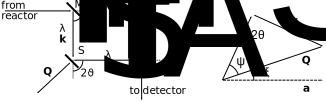
\includegraphics[width = 0.75 \textwidth]{figures/tas_triangle}
	\end{center}
	\caption[TAS layout and scattering triangle.]{
		Triple-axis layout (left) and scattering triangle (right). \label{fig:scattering_triangle}}
\end{figure}

We can calculate $2 \theta_S$ by forming the scalar product of $\left| Q \right>$ with itself.
\begin{equation} 
	\left| Q \right> \ =\  \left| k_i \right> - \left| k_f \right> \\ 
\end{equation}
\begin{equation} 
	\left< Q | Q \right> \ =\  \left( \left< k_i \right| - \left< k_f \right| \right) \cdot \left( \left| k_i \right> - \left| k_f \right> \right)
\end{equation}
\begin{equation} 
	\left< Q | Q \right> \ =\  \left< k_i | k_i \right> + \left< k_f | k_f \right> - 2 \left< k_i | k_f \right> 
\end{equation}
\begin{equation} 
	Q^2 \ =\  k_i^2 + k_f^2 - 2 k_i k_f \cos \left( 2 \theta_S \right) 
\end{equation}
\begin{equation}
	\boxed{ 2 \theta_S \ =\  \sigma_s \cdot \arccos \left( \frac{k_i^2 + k_f^2 - Q^2}{2 k_i k_f} \right) } 
\end{equation}

As we could scatter in either clockwise or counterclockwise direction, $2 \theta_S$ can be positive or negative.
The sign of $2 \theta_S$ is given by the sample scattering sense $\sigma_s = \pm 1$.


\vspace{0.5cm}


The final and most complicated angle to determine is the sample rotation $\Theta_S$.
It is given by the angle of the incoming wavevector $\left| k_i \right>$ to an (arbitrary) direction $\left| a \right>$ which is known from sample orientation, this is usually a Bragg peak. If we were to explicitly use the $U$ matrix here, this vector would be one of its rows.
The situation is shown in the right panel of Fig. \ref{fig:scattering_triangle}.
We split $\Theta_S$ into the angle $\psi$ between $\left| k_i \right>$ and $\left| Q \right>$ and the angle $\xi$ between $\left| k_i \right>$ and $\left| a \right>$:
\begin{equation} \boxed{ \Theta_S \ =\  180^{\circ} - \left( \psi + \xi \right) } \end{equation}


\vspace{0.5cm}


The angle $\psi$ between $\left| k_i \right>$ and $\left| Q \right>$ is determined from the scattering triangle, as before:
\begin{equation}
	\left| k_f \right> \ =\  \left| k_i \right> - \left| Q \right> 
\end{equation}
\begin{equation} 
	\left< k_f | k_f \right> \ =\  \left( \left< k_i \right| - \left< Q \right| \right) \cdot \left( \left| k_i \right> - \left| Q \right> \right)
\end{equation}
\begin{equation}
	\left< k_f | k_f \right> \ =\  \left< k_i | k_i \right> + \left< Q | Q \right> - 2 \left< k_i | Q \right>
\end{equation}
\begin{equation}
	k_f^2 \ =\  k_i^2 + Q^2 - 2 k_i Q \cos \psi 
\end{equation}
\begin{equation}
	\boxed{ \psi \ =\  \sigma_s \cdot \arccos \left( \frac{k_i^2 + Q^2 - k_f^2}{2 k_i Q} \right) }
\end{equation}


\vspace{0.5cm}


The angle $\xi$ between $\left| Q \right>$ and orientation vector $\left| a \right>$ is also determined from the properties of the scalar product.
Here we have to use the covariant form, because $\left| a \right>$ is a coordinate in crystal space naming a Bragg reflection, while $\left| Q \right>$ lives, as before in instrument space.
\begin{equation} 
	\boxed{ \xi \ =\  
\sigma_{\mathrm{side}} \cdot \arccos \left( \frac{ \left< Q | a \right> }{ \sqrt{\left< Q | Q \right>} \sqrt{\left< a | a \right>} } \right) \ =\  
\sigma_{\mathrm{side}} \cdot \arccos \left( \frac{ Q^i g_{ij} a^j }{ \sqrt{Q^i g_{ij} Q^j} \sqrt{a^i g_{ij} a^j} } \right) } 
\label{eq:xi}
\end{equation}

The sign, $\sigma_{\mathrm{side}}$, of $\xi$ depends on which side of the orientation vector $\left| a \right>$ the scattering vector $\left| Q \right>$ is located. 
The sign can be found by calculating the (covariant) cross product of $\left| a \right>$ and $\left| Q \right>$ to give an out-of-plane vector $\left| x \right>$ which can be compared with the given scattering plane up vector.
The covariant cross-product is calculated as \cite[p. 815]{Arens2015}:
\begin{equation}
	x^l \ =\  g^{li} \epsilon_{ijk} a^j Q^k,
\end{equation}
where $\epsilon_{ijk}$ is the general Levi-Civita symbol formed from the determinant of the basis vectors $\left| \underline{b}_i \right>$, see Ref. \cite[p. 815]{Arens2015}:
\begin{equation}
	\epsilon_{ijk} \ =\  \left|
		\begin{array}{ccc} \left| 
			\underline{b}_i \right> & \left| \underline{b}_j \right> & \left| \underline{b}_k \right>
		\end{array} \right|.
\end{equation}



\paragraph*{Special case}
For cubic crystals with $\alpha = \beta = \gamma = 90^{\circ}$ and the lattice constants all equal, $a = b = c$, the metric tensor is diagonal, $g_{ij} = \delta_{ij} \cdot \left( 2\pi / a \right)^2$.
With that, Eq. \ref{eq:xi} simplifies to:
\begin{equation}
	\xi \ =\  \sigma_{\mathrm{side}} \cdot \arccos \left( \frac{ Q_i a^i }{ \sqrt{Q_i Q^i} \sqrt{a_i a^i} } \right).
\end{equation}
% ------------------------------------------------------------------------------------------------------------------------------------


\section{Summary}
TODO


\chapter{Path-finding}
%
% path-finding
% @author Tobias Weber <tweber@ill.fr>
% @date 2021
% @license see 'LICENSE' file
%

This chapter is devoted to the development of the theoretical frameworks for path-finding in a triple-axis spectrometer (TAS). 
The path should furthermore be optimal in the sense that the instrument not only avoids obstacles like walls or equipment in 
the experimental area, but also keeps a maximum distance from them.

Before looking at the situation with TAS in section \ref{sec:tasrobot}, we review the ideas of motion planning for a point-like robot.



\section{Motion planning for a point-like robot}
\label{sec:pointrobot}

The algorithm for motion planning in a point-like robot are given in Ref. \cite[Ch. 13, pp. 283-306]{Berg2008}, whose descriptions 
we follow in this section. While the book chapter also describes polygonal robots, we limit ourselves to the parts of the chapter 
that are relevant for the present work.





\section{Motion planning for a triple-axis spectrometer}
\label{sec:tasrobot}

% TODO: moving instrument along voronoi edges


\chapter{Implementation}
% library
% GUI
% Nomad interface
% Verweis auf Nomad 3D und vTAS/vEXP


\appendix
%\part{Back matter}
%\addcontentsline{toc}{part}{Back matter} 
%
% notation
% @author Tobias Weber <tweber@ill.fr>
% @date mar-2021
% @license see 'LICENSE' file
%

\chapter{Notation}

\begin{tabular}{|c|c|}
\hline
\bf{Notation} & \bf{Explanation} \tabularnewline
\hline
$ \underline{v} $ & A vector. \tabularnewline
\hline
$ M = \left( m_{ij} \right) $ & A matrix. \tabularnewline
\hline
$\left| x \right> \,=\, \left( x^i \right) $ & A contravariant vector. \tabularnewline
\hline
$\left< x \right| \,=\, \left( x_i \right) $ & A covariant vector. \tabularnewline
\hline
$s \,=\, \left< x | y \right> \,=\, x_i y^i \,=\, g_{ij} x^i y^j $ & A scalar/inner product, the sums over $i$ and $j$ are implied \cite{wiki_summation}. \tabularnewline
\hline
$\left(a^{i}_{\;j}\right) \,=\, \left| x \right> \left< y \right| \,=\, x^i y_j$ & A tensor/outer product. \tabularnewline
\hline
\end{tabular}

%
% publication list
% @author Tobias Weber <tweber@ill.fr>
% @date july-2021
% @license see 'LICENSE' file
%

\chapter{List of Publications}
The latest list of publications can be found on-line under \url{https://orcid.org/0000-0002-7230-1932}. 
We reproduce the current version as of July 2021 in the following.


\section{Works as principal author}
\subsection*{Papers}
\begin{itemize}
	\item T. Weber, D. M. Fobes, J. Waizner, P. Steffens, G. S. Tucker,
	M. B\"ohm, L. Beddrich, C. Franz, H. Gabold, R. Bewley,
	D. Voneshen, M. Skoulatos, R. Georgii, G. Ehlers, A. Bauer,
	C. Pfleiderer, P. B\"oni, M. Janoschek, and M. Garst, 
	\textit{Emergent Landau levels of magnons in a skyrmion lattice},
	submitted, in review.

	\item T. Weber, \textit{Update 2.0 to ``Takin: An open-source software for experiment planning, visualisation, and data analysis'', (PII: S2352711016300152)},
	SoftwareX, Volume 14, 100667 (June 2021),
	DOI: \href{https://doi.org/10.1016/j.softx.2021.100667}{10.1016/j.softx.2021.100667}.

	\item T. Weber, J. Waizner, P. Steffens, A. Bauer, C. Pfleiderer, M. Garst, and P. B\"oni, 
	\textit{Polarized inelastic neutron scattering of nonreciprocal spin waves in MnSi},
	Physical Review B, Volume 100, 060404(R) (12 August 2019),
	DOI: \href{https://doi.org/10.1103/PhysRevB.100.060404}{10.1103/PhysRevB.100.060404}.

	\item  T. Weber, J. Waizner, G. S. Tucker, L. Beddrich, M. Skoulatos, R. Georgii, A. Bauer, C. Pfleiderer, M. Garst, and P. B\"oni, 
	\textit{Non-reciprocal magnons in non-centrosymmetric MnSi},
	AIP Advances, Volume 8, 101328 (9 October 2018),
	DOI: \href{https://doi.org/10.1063/1.5041036}{10.1063/1.5041036}.

	\item T. Weber, J. Waizner, G. S. Tucker, R. Georgii, M. Kugler, A. Bauer, C. Pfleiderer, M. Garst, and P. B\"oni, 
	\textit{Field dependence of nonreciprocal magnons in chiral MnSi},
	Physical Review B, Volume 97, 224403 (5 June 2018),
	DOI: \href{https://doi.org/10.1103/PhysRevB.97.224403}{10.1103/PhysRevB.97.224403}.

	\item T. Weber, B. Roessli, C. Stock, T. Keller, K. Schmalzl, F. Bourdarot, R. Georgii, R. A. Ewings, R. S. Perry, and P. B\"oni, 
	\textit{Transverse acoustic phonon anomalies at intermediate wave vectors in $MgV_2O_4$},
	Physical Review B, Volume 96, 184301 (7 November 2017),
	DOI: \href{https://doi.org/10.1103/PhysRevB.96.184301}{10.1103/PhysRevB.96.184301}.
	
	\item T. Weber, \textit{Update 1.5 to ``Takin: An open-source software for experiment planning, visualisation, and data analysis'', (PII: S2352711016300152)},
	SoftwareX, Volume 6, Pages 148-149 (10 July 2017),
	DOI: \href{https://doi.org/10.1016/j.softx.2017.06.002}{10.1016/j.softx.2017.06.002}.

	\item T. Weber, R. Georgii, and P. B\"oni,
	\textit{Takin: An open-source software for experiment planning, visualisation, and data analysis},
	SoftwareX, Volume 5, Pages 121-126 (14 July 2016),
	DOI: \href{https://doi.org/10.1016/j.softx.2016.06.002}{10.1016/j.softx.2016.06.002}.

	\item T. Weber, G. Brandl, R. Georgii, and P. B\"oni,
	\textit{An open-source software package for data treatment in a MIEZE experiment},
	Journal of Physics: Conference Series, Volume 528, 012034 (2014),
	DOI: \href{https://doi.org/10.1088/1742-6596/528/1/012034}{10.1088/1742-6596/528/1/012034}.
	
	\item T. Weber, G. Brandl, R. Georgii, W. H\"au\ss{}ler, S. Weichselbaumer, P. B\"oni,
	\textit{Monte-Carlo simulations for the optimisation of a TOF-MIEZE instrument},
	Nuclear Instruments and Methods in Physics Research Section A: Accelerators, Spectrometers, Detectors and Associated Equipment, Volume 713, Pages 71-75 (11 June 2013),
	DOI: \href{https://doi.org/10.1016/j.nima.2013.03.010}{10.1016/j.nima.2013.03.010}.
\end{itemize}


\subsection*{Theses}
\begin{itemize}
	\item T. Weber, \textit{Dynamics at the Orbital Ordering Phase Transition in $MgV_2O_4$ and at the Ferromagnetic Phase Transition in $MnSi$} (20 March 2017), ISBN: 978-3-8439-3114-4,
	PhD Thesis in Physics, Technische Universit\"at M\"unchen, Physikdepartment E21,
	Garching bei M\"unchen, Germany. URL: \url{http://nbn-resolving.de/urn/resolver.pl?urn:nbn:de:bvb:91-diss-20170320-1339645-0-4}.

	\item T. Weber, \textit{MIEZE in Theory, Simulation and Experiment} (5 December 2012), 
	Diploma Thesis in Physics, Technische Universit\"at M\"unchen, Physikdepartment E21,
	Garching bei M\"unchen, Germany.
\end{itemize}



\section{Works as contributing author}

\begin{itemize}
	\item M. M. Noack, P. H. Zwart, D. M. Ushizima, M. Fukuto, K. G. Yager, K. C. Elbert, 
		C. B. Murray, A. Stein, G. S. Doerk, E. H. R. Tsai, R. Li, G. Freychet, 
		M. Zhernenkov, H.-Y. N. Holman, S. Lee, L. Chen, E. Rotenberg, T. Weber, 
		Y. Le Goc, M. B\"ohm, P. Steffens, P. Mutti, and J. A. Sethian, 
	\textit{Gaussian processes for autonomous data acquisition at large-scale synchrotron and neutron facilities},
	Nature Review Physics (28 July 2021),
	DOI: \href{https://doi.org/10.1038/s42254-021-00345-y}{10.1038/s42254-021-00345-y}.

	\item Y. Nambu, J. Barker, Y. Okino, T. Kikkawa, Y. Shiomi, M. Enderle, T. Weber, B. Winn, M. Graves-Brook, J. M. Tranquada, T. Ziman, M. Fujita, G. E. W. Bauer, E. Saitoh, and K. Kakurai, 
	\textit{Observation of Magnon Polarization},
	Physical Review Letters, Volume 125, 027201 (6 July 2020),
	DOI: \href{https://doi.org/10.1103/PhysRevLett.125.027201}{10.1103/PhysRevLett.125.027201}.

	\item G. Song, L. Porcar, M. B\"ohm, F. Cecillon, C. Dewhurst, Y. Le Goc, J. Locatelli, P. Mutti, and T. Weber, 
	\textit{Deep Learning Methods On Neutron Scattering Data},
	EPJ Web of Conferences, Volume 225, 01004 (20 January 2020),
	DOI: \href{https://doi.org/10.1051/epjconf/202022501004}{10.1051/epjconf/202022501004}.

	\item D. W. Tam, H.-H. Lai, J. Hu, X. Lu, H. C. Walker, D. L. Abernathy, J. L. Niedziela, T. Weber, M. Enderle, Y. Su, Z. Q. Mao, Q. Si, and P. Dai,
	\textit{Plaquette instability competing with bicollinear ground state in detwinned FeTe},
	Physical Review B, Volume 100, 054405 (5 August 2019),
	DOI: \href{https://doi.org/10.1103/PhysRevB.100.054405}{10.1103/PhysRevB.100.054405}.
	
	\item R. Georgii and T. Weber,
	\textit{The Helical Magnet MnSi: Skyrmions and Magnons},
	Quantum Beam Science 2019, Volume 3(1) (21 February 2019),
	DOI: \href{https://doi.org/10.3390/qubs3010004}{10.3390/qubs3010004}.
	
	\item R. Georgii, T. Weber, G. Brandl, M. Skoulatos, M. Janoschek, S. Mühlbauer, C. Pfleiderer, and P. B\"oni,
	\textit{The multi-purpose three-axis spectrometer (TAS) MIRA at FRM II},
	Nuclear Instruments and Methods in Physics Research Section A: Accelerators, Spectrometers, Detectors and Associated Equipment, Volume 881, Pages 60-64 (11 February 2018),
	DOI: \href{https://doi.org/10.1016/j.nima.2017.09.063}{10.1016/j.nima.2017.09.063}.
\end{itemize}

%
% future errata
% @author Tobias Weber <tweber@ill.fr>
% @date july-2021
% @license see 'LICENSE' file
%

\chapter{Accompanying Software and Future Errata}
\label{ch:online}

\paragraph{Software source code}
The latest version the software that has been developed 
as part of this work has the DOI (digital object identifier)
\href{https://doi.org/10.5281/zenodo.4625649}{10.5281/zenodo.4625649}
and can be found under the URL \url{https://doi.org/10.5281/zenodo.4625649}.
The source code is also provided on the supplementary medium (CD-ROM and/or USB drive) 
attached to this work, together with compiled versions.

Additionally, the main software's development repository is available here: 
\url{https://code.ill.fr/scientific-software/takin/paths},
a mirror of the repository can be found here: 
\url{https://github.com/tweber-ill/ill_mirror-takin2-paths}.
It has furthermore been permanently archived at the address:
\url{https://archive.softwareheritage.org/browse/origin/?origin_url=https://code.ill.fr/scientific-software/takin/paths}.

The latest version of the software's source code archive (ver-1.1) bears the
filename ``taspaths-oct21d.tar.xz'' and has the SHA-256 \cite{web_sha256sum}
checksum:

\begin{centering}
\texttt{\\
58cf3b96c9abc6d5\phantom{.} \\
4bdefc12dcd38aa1\phantom{.} \\
db2e8708d5bc7294\phantom{.} \\
03054e44286547ec.}\\
\end{centering}


\paragraph{Source code layout}
The layout of the software's source code archive is shown in table \ref{tab:sourcelayout}.

\begin{table}[htb]
	\centering
	\begin{tabular}{|c c|c|c|}
		\hline
		\bf{Folder} & & \bf{Explanation} & \bf{References} \tabularnewline
		\hline
		src/ & & Main source directory. & \tabularnewline
		       & libs/ & Library of geometry algorithms and data structures. & Chapter \ref{ch:algos}. \tabularnewline
		       & core/ & Core TAS path finding library. & Chapters \ref{ch:impl} and \ref{sec:library}. \tabularnewline
		       & gui/ & Graphical user interface and 3-D editor/viewer. & Chapter \ref{sec:gui}. \tabularnewline
		       & tools/ & Helper and auxiliary tools. & Chapter \ref{sec:tests_tools}. \tabularnewline
		\hline
		scripting/ & & Python scripting interface. & Chapter \ref{sec:scripting} \tabularnewline
		\hline
		unittests/ & & Unit tests. & Chapter \ref{sec:unit_tests}. \tabularnewline
		\hline
		tests/ & & Small (performance) test programs. & \tabularnewline
		\hline
		res/ & & Resource files, e.g. shader scripts. & \tabularnewline
		\hline
		cmake/ & & Modules for the \textit{CMake} \cite{Martin2007, web_cmake} build system. & \tabularnewline
		\hline
		setup/ & & Compile and setup scripts for... & \tabularnewline
		           & osx/ & ... \textit{MacOS} using \textit{Homebrew} \cite{web_homebrew}, & \tabularnewline
		           & deb/ & ... \textit{GNU/Linux}, mainly \textit{Ubuntu}, & \tabularnewline
		           & mingw/ & ... \textit{MinGW} \cite{web_mingw64}. & \tabularnewline
		\hline
		tlibs2/ & & Mathematical template library developed  & \cite{Takin2016, Takin2017, Takin2021, DiplomaWeber, PhDWeber} \tabularnewline
		           & & during my physics diploma and doctoral theses. & \tabularnewline
		\hline
		externals/ & & Further external library dependencies. & \tabularnewline
		\hline
	\end{tabular}
	\caption[Source code layout.]{Layout of the source code.}
	\label{tab:sourcelayout}
\end{table}

Development of the geometry library under \lstinline|./src/libs| and the auxiliary tools under \lstinline|./src/tools| 
was already started in 2020, as preparation for the exam in Algorithmic Geometry, and their source code 
is therefore based on the course materials \cite{FUH_geo2020}. 
Afterwards, the library and tools have been further developed for this work, their separate code repository is available under 
\url{https://github.com/t-weber/geo}, the software is furthermore registered under the DOI 
\href{https://doi.org/10.5281/zenodo.4297475}{10.5281/zenodo.4297475}.

This software is based on the \textit{tlibs} libraries, which reside in the 
sub-directory \lstinline|./tlibs2|, but are not part of the present thesis.
That library has already been developed since my diploma thesis \cite{DiplomaWeber} 
and my doctoral thesis \cite{PhDWeber}, as well as during several software 
projects \cite{Weber2014, Takin2016, Takin2017, Takin2021}.
Its full source code is included in the source archive merely for the convenience of not
having to search the correct version.
Apart from using the \textit{tlibs} library, several code snippets are further developments
of their counterparts from that library and the \textit{Takin} project \cite{Takin2021, Takin2017, Takin2016} in general, 
among these the setup and build scripts for the various systems, 
as well as the \textit{OpenGL} renderer and general-purpose code.
The \textit{OpenGL} renderer was furthermore based on example source code \cite{web_QOpenGLWidgetExampleThreaded} provided
with the \textit{Qt} \cite{web_Qt} library.


\paragraph{Thesis source code}
The source of the thesis text can be found in the repository:
\url{https://code.ill.fr/tweber/thesis}, and is mirrored in:
\url{https://github.com/tweber-ill/ill_mirror-thesis}.
The archived copy of the repository can be found here:
\url{https://archive.softwareheritage.org/browse/origin/?origin_url=https://code.ill.fr/tweber/thesis}.

%The thesis has the DOI \href{https://doi.org/TODO}{TODO}
%and can be found under the URL \url{https://doi.org/TODO}.


%\vspace{0.75cm}
\paragraph{Errata}
Up-to-date errata for this work will be published via the DOI
\href{https://doi.org/10.5281/zenodo.5092159}{10.5281/zenodo.5092159}
and can be found online under the URL \url{https://doi.org/10.5281/zenodo.5092159}.


%\section{Bibliography}
\bibliographystyle{ieeetr}
\bibliography{\jobname.bib}
% ====================================================================================================================================

\end{document}
